% Closer description of poject

\section{Project Description}
Robots like SiA20 Motoman are powerful and can in some situations cause harm to humans working in the same area. The goal of this project is to create a system which ensures a safe environment in a human robot collaboration area. This will be done by determining the distance between the closest moving object and the robot and retrieve a control signal to send to the robot depending on that information. The control signal should determine four states:
\begin{enumerate}
\item The closest moving object is outside safety zone 2 (see figure below). Objects are not in the collaborative area, the robot can work at standard motion. 

\item The closest moving object is within safety zone 2. This means that the robot motion shall be reduced since the moving object is within the collaborative area.

\item The closest moving object is within safety zone 1. This means that the robot must stop.

\item The closest moving object is within the emergency zone. This means that the robot must perform an emergency stop, which differs from the usual stop. 
\end{enumerate}

\begin{figure}[H]
\begin{center}
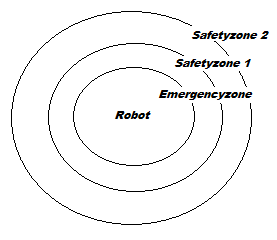
\includegraphics[width=7 cm]{robotsafetyzone}
\caption{Flowchart of tracking algorithm}
\label{robotsafetyzone}
\end{center}
\end{figure}
